\section{Auswertung}
\label{sec:auswertung}
	Im Folgenden werden einige Mittelwerte gebildet.
	Bei einer Anzahl von $n$ Messwerten $x_\mathrm{i}$ gilt f"ur den Mittelwert $x$:

	\begin{equation*}
		x = \frac{1}{n} \sum_{\mathrm{i} = 0}^n {x_\mathrm{i}} \,.
	\end{equation*}

	Die Varianz $\sigma_x$ dieses Wertes, bzw. dessen Fehler $\Delta x$ betragen

	\begin{equation*}
		\Delta x^2 = \sigma_x = \frac{1}{n - 1} \sum_{\mathrm{i} = 0}^n{\left(x_\mathrm{i} - x\right)^2} \,.
	\end{equation*}

	\subsection{Bestimmung der mittleren Reichweite $R_\mathrm{m}$ mit der entsprechenden Energie $E_\mathrm{m}$}
	\label{subsec:mittlere_reichweite}
		Zur Ermittlung der mittleren Reichweite $R_\mathrm{m}$ wird die Z"ahlrate $z$ gegen die effektive L"ange $x_\mathrm{eff}$ aufgetragen.
		Durch die abfallende Flanke (siehe Abbildungen \ref{fig:zaehlrate1} und \ref{fig:zaehlrate2}) wird eine lineare Ausgleichsgerade der Form $z(x) = mx + b$ gelegt.
		Die mittlere Reichweite $R_\mathrm{m}$ entspricht der x-Koordinate dieser Ausgleichgerade an der Stelle der halben, maximalen Z"ahlrate $z_\mathrm{max}$.

		Es gilt also

		\begin{equation*}
			R_\mathrm{m} = \frac{\frac{z_\mathrm{max}}{2} - b}{m} \,.
		\end{equation*}

		Die maximale Energie $E$, die bei einer Messung detektiert wird, ist proportional zum gemessenen Kanal $c$.
		Mit Kenntnis der Energie $E_\mathrm{max}$ bei einer bestimmten L"ange $x_\mathrm{eff}$ lassen sich somit alle Energiewerte berechnen.

		Die Messwerte der beiden Messungen sind in den Tabellen \ref{table:messung1-1} und \ref{table:messung1-2} aufgef"uhrt.
		Die Werte, die zur Ausgleichsrechnung benutzt werden, sind farbig \textcolor{red}{rot} markiert.

		\clearpage
		Die Ausgleichsrechnung durch \emph{python} der ersten Messreihe bei $x_{0,2} = \SI{2.6}{\centi \meter}$ liefert
		% \begin{table}[h!]
		% 	\begin{center}
		% 		\begin{tabular}{rclcrcl}
		% 			$m$ & $=$ & $\SI{-1120(8)}{\per \second \per \centi \per \meter}$ & $,$ & $b$ & $=$ & $\SI{2657(16)}{\per \second}$\\
		% 			\hspace{.2cm} \\
		% 			$\Rightarrow R_\mathrm{m}$ & $=$ & $\SI{2.13(2)}{\centi \meter}$ & $,$ & $E_\mathrm{m}$ & $=$ & $\SI{1.65(15)}{\mega \electronvolt}$\\
		% 		\end{tabular}
		% 	\end{center}
		% \end{table}
		\begin{eqnarray*}
			m_1 = \SI{-1120(8)}{\per \second \per \centi \per \meter} &,& b_1 = \SI{2657(16)}{\per \second} \\
			\Rightarrow R_\mathrm{m,1} = \SI{2.13(2)}{\centi \meter} &,& E_\mathrm{m,1} = \SI{1.65(15)}{\mega \electronvolt} \,,
		\end{eqnarray*}

		sowie bei $x_{0,1} = \SI{2.8}{\centi \meter}$
		\begin{eqnarray*}
			m_2 = \SI{-1115(60)}{\per \second \per \centi \per \meter} &,& b_2 = \SI{2648(129)}{\per \second} \\
			\Rightarrow R_\mathrm{m,2} = \SI{2.14(16)}{\centi \meter} &,& E_\mathrm{m,2} = \SI{1.67(8)}{\mega \electronvolt} \,.
		\end{eqnarray*}

		Die Abbildungen \ref{fig:zaehlrate1} und \ref{fig:zaehlrate2} beinhalten die entsprechenden Kurven dieser Messung.

		\begin{table}[h!]
			\begin{center}
				\caption{Messwerte bei Basisl"ange $x_{0,1}$ und einer Messzeit $T = \SI{120}{\second}$ \label{table:messung1-1}}
				\begin{tabular}{|r|r|r|r|r|}
					\hline
						\multicolumn{1}{|c|}{$p [\SI{}{\milli \bar}]$}& 
						\multicolumn{1}{c|}{Counts} & 
						\multicolumn{1}{c|}{$z \left[\SI{}{\per \second}\right]$} & 
						\multicolumn{1}{c|}{Channel $c$} & 
						\multicolumn{1}{c|}{$E [\SI{}{\mega \electronvolt}]$} \\
					\hline 
					\hline
						\SI{0000}{} & \SI{64755}{} &\SI{539.63}{}  & \SI{2336}{} & \textcolor{blue}{\SI{4.000}{}} \\
\SI{0100}{} & \SI{63966}{} &\SI{533.05}{}  & \SI{2112}{} & \textcolor{blue}{\SI{3.616}{}} \\
\SI{0200}{} & \SI{63083}{} &\SI{525.69}{}  & \SI{2047}{} & \textcolor{blue}{\SI{3.505}{}} \\
\SI{0300}{} & \SI{62009}{} &\SI{516.74}{}  & \SI{1835}{} & \textcolor{blue}{\SI{3.142}{}} \\
\SI{0400}{} & \SI{60962}{} &\SI{508.02}{}  & \SI{1691}{} & \textcolor{blue}{\SI{2.896}{}} \\
\SI{0450}{} & \SI{60035}{} &\SI{500.29}{}  & \SI{1631}{} & \textcolor{blue}{\SI{2.793}{}} \\
\SI{0500}{} & \SI{59706}{} &\SI{497.55}{}  & \SI{1536}{} & \textcolor{blue}{\SI{2.630}{}} \\
\SI{0550}{} & \SI{58693}{} &\SI{489.11}{}  & \SI{1491}{} & \textcolor{blue}{\SI{2.553}{}} \\
\SI{0600}{} & \SI{57238}{} &\SI{476.98}{}  & \SI{1391}{} & \textcolor{blue}{\SI{2.382}{}} \\
\SI{0650}{} & \SI{55828}{} &\SI{465.23}{}  & \SI{1295}{} & \textcolor{blue}{\SI{2.217}{}} \\
\SI{0700}{} & \SI{53848}{} &\SI{448.73}{}  & \SI{1023}{} & \textcolor{blue}{\SI{1.752}{}} \\
\SI{0750}{} & \SI{50700}{} &\SI{422.50}{}  & \SI{0984}{} & \textcolor{blue}{\SI{1.685}{}} \\
\SI{0800}{} & \SI{42840}{} &\textcolor{red}  {\SI{357.00}{}}  & \SI{0844}{} & \SI{1.445}{} \\
\SI{0850}{} & \SI{25797}{} &\textcolor{red}  {\SI{214.97}{}}  & \SI{0727}{} & \SI{1.245}{} \\
\SI{0900}{} & \SI{08352}{} &\textcolor{red}  {\SI{069.60}{}}  & \SI{0655}{} & \SI{1.122}{} \\
\SI{0950}{} & \SI{02920}{} &                  \SI{024.33}{}   & \SI{0652}{} & \SI{1.116}{} \\
\SI{1000}{} & \SI{00053}{} &                  \SI{000.44}{}   & \SI{0678}{} & \SI{1.161}{} \\
					\hline 
				\end{tabular}
			\end{center}
		\end{table}

		\begin{table}[h!]
			\begin{center}
				\caption{Messwerte bei Basisl"ange $x_{0,2}$ und einer Messzeit $T = \SI{120}{\second}$ \label{table:messung1-2}}
				\begin{tabular}{|r|r|r|r|r|}
					\hline
						\multicolumn{1}{|c|}{$p [\SI{}{\milli \bar}]$}& 
						\multicolumn{1}{c|}{Counts} & 
						\multicolumn{1}{c|}{$z \left[\SI{}{\per \second}\right]$} & 
						\multicolumn{1}{c|}{Channel $c$} & 
						\multicolumn{1}{c|}{$E [\SI{}{\mega \electronvolt}]$} \\
					\hline 
					\hline
						\SI{0000}{} & \SI{64243}{} &\SI{535.36}{} & \SI{2319}{} & \textcolor{blue}{\SI{4.000}{}} \\
\SI{0100}{} & \SI{64005}{} &\SI{533.38}{} & \SI{2112}{} & \textcolor{blue}{\SI{3.643}{}} \\
\SI{0200}{} & \SI{62870}{} &\SI{523.92}{} & \SI{1999}{} & \textcolor{blue}{\SI{3.448}{}} \\
\SI{0300}{} & \SI{61075}{} &\SI{508.96}{} & \SI{1839}{} & \textcolor{blue}{\SI{3.172}{}} \\
\SI{0400}{} & \SI{60439}{} &\SI{503.66}{} & \SI{1711}{} & \textcolor{blue}{\SI{2.951}{}} \\
\SI{0450}{} & \SI{60471}{} &\SI{503.93}{} & \SI{1583}{} & \textcolor{blue}{\SI{2.730}{}} \\
\SI{0500}{} & \SI{58985}{} &\SI{491.54}{} & \SI{1543}{} & \textcolor{blue}{\SI{2.661}{}} \\
\SI{0550}{} & \SI{57953}{} &\SI{482.94}{} & \SI{1431}{} & \textcolor{blue}{\SI{2.468}{}} \\
\SI{0600}{} & \SI{57250}{} &\SI{477.08}{} & \SI{1359}{} & \textcolor{blue}{\SI{2.344}{}} \\
\SI{0650}{} & \SI{55154}{} &\SI{459.62}{} & \SI{1276}{} & \textcolor{blue}{\SI{2.201}{}} \\
\SI{0700}{} & \SI{53891}{} &\SI{449.09}{} & \SI{1103}{} & \textcolor{blue}{\SI{1.903}{}} \\
\SI{0750}{} & \SI{49951}{} &\SI{416.26}{} & \SI{1023}{} & \textcolor{blue}{\SI{1.765}{}} \\
\SI{0800}{} & \SI{42639}{} &\textcolor{red}{\SI{355.32}{}}& \SI{0762}{} & \SI{1.314}{} \\
\SI{0850}{} & \SI{27054}{} &\textcolor{red}{\SI{225.45}{}}& \SI{0655}{} & \SI{1.130}{} \\
\SI{0900}{} & \SI{08309}{} &\textcolor{red}{\SI{069.24}{}}& \SI{0652}{} & \SI{1.125}{} \\
\SI{0950}{} & \SI{02838}{} &                \SI{023.65}{} & \SI{0664}{} & \SI{1.145}{} \\
\SI{1000}{} & \SI{00049}{} &                \SI{000.41}{} & \SI{0723}{} & \SI{1.247}{} \\
					\hline 
				\end{tabular}
			\end{center}
		\end{table}

		\begin{figure}[h]
			\centering
			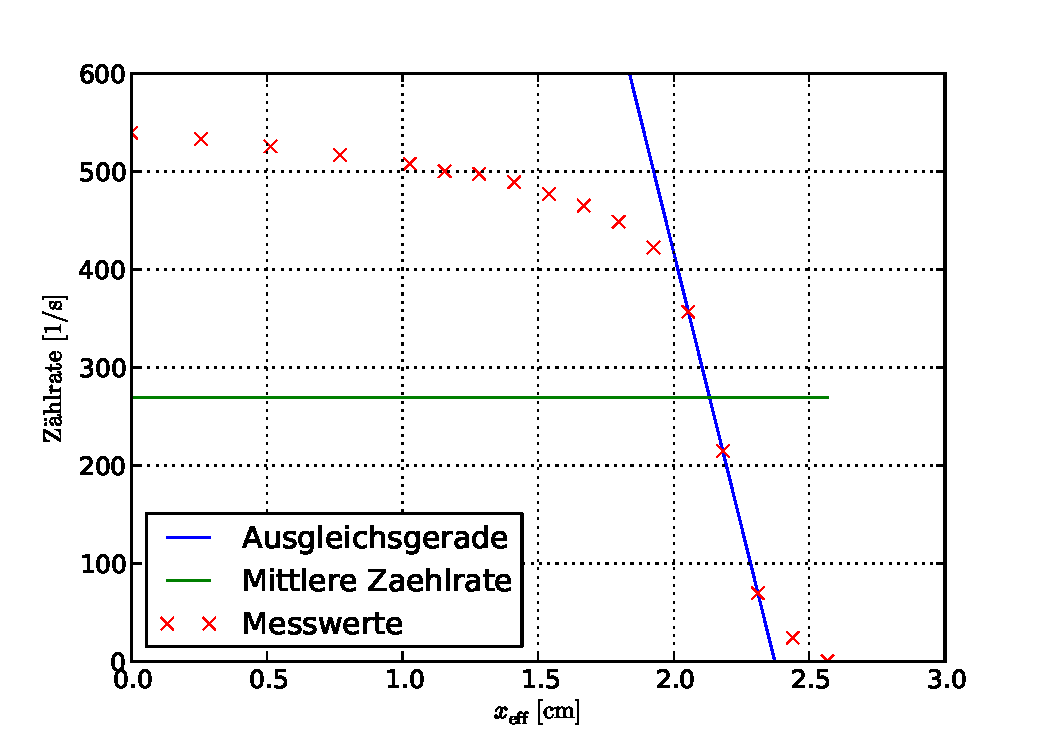
\includegraphics[width = 13cm]{img/zaehlrate1.pdf}
			\caption{Graph zur Bestimmung der mittleren Reichweite $R_\mathrm{m}$ bei Basisl"ange $x_{0,1}$ \label{fig:zaehlrate1}}
		\end{figure}

		\begin{figure}[h]
			\centering
			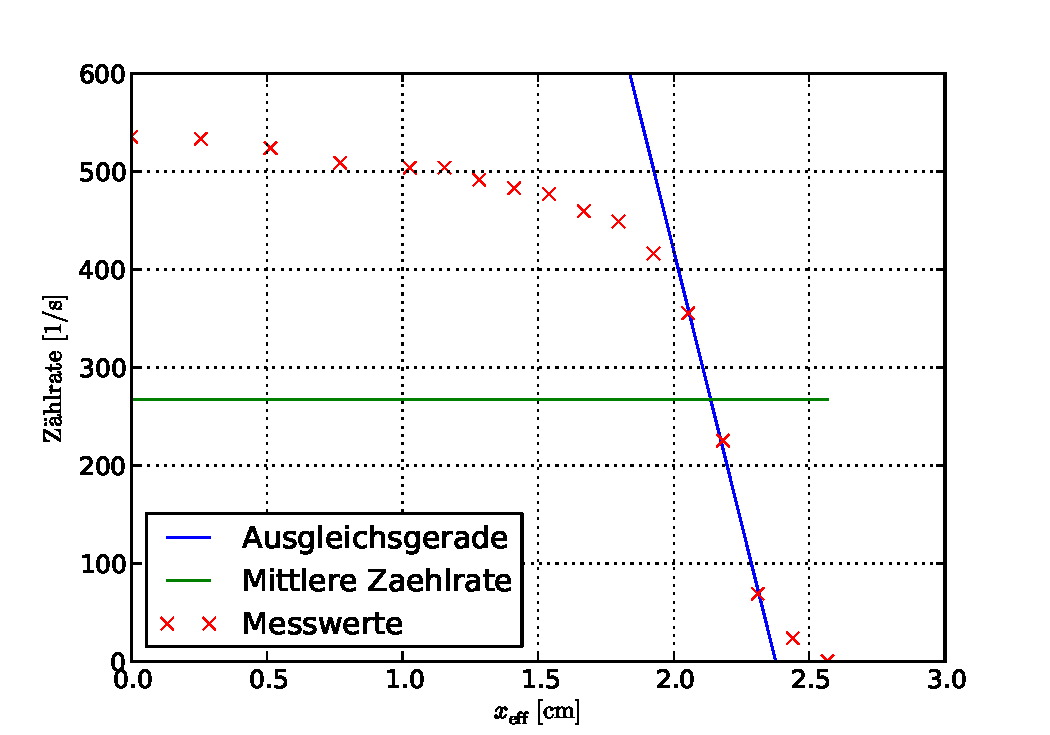
\includegraphics[width = 15cm]{img/zaehlrate2.pdf}
			\caption{Graph zur Bestimmung der mittleren Reichweite $R_\mathrm{m}$ bei Basisl"ange $x_{0,2}$ \label{fig:zaehlrate2}}
		\end{figure}

		\clearpage

	\subsection{Energieverlust $-\mathrm{d}E$ pro Weg $\mathrm{d}x$}
	\label{subsec:energieverlust}
		Tr"agt man die in Tabellen \ref{table:messung1-1} und \ref{table:messung1-2} aufgef"uhrten Energien $E$ gegen die effektive L"ange $x_\mathrm{eff}$ auf, l"asst sich der Energieverlust $-\mathrm{d}E / \mathrm{d}x$ durch eine lineare Ausgleichsgerade der Form $E(x) = mx + b$ bestimmen.
		Die Steigung $m$ entspricht hierbei dem Energieverlust $\mathrm{d}E / \mathrm{d}x$.

		Die Ausgleichsrechnung durch \emph{python} liefert

		\begin{equation*}
			-\frac{\mathrm{d}E}{\mathrm{d}x} = \SI{1.10944(606)}{\mega \electronvolt \per \centi \meter}
		\end{equation*}

		f"ur die Messung bei der Basisl"ange $x_{0,1}$ und

		\begin{equation*}
			-\frac{\mathrm{d}E}{\mathrm{d}x} = \SI{1.10938(335)}{\mega \electronvolt \per \centi \meter}
		\end{equation*}

		f"ur die Messung bei der Basisl"ange $x_{0,1}$.

		Die entsprechenden Graphen sind in Abbildung \ref{fig:energie1} und \ref{fig:energie2} dargestellt.
		Die zur Ausgleichsrechnung benutzten Messwerte sind in Tabellen \ref{table:messung1-1} und \ref{table:messung1-2} \textcolor{blue}{blau} gekennzeichnet.

		\begin{figure}[h]
			\centering
			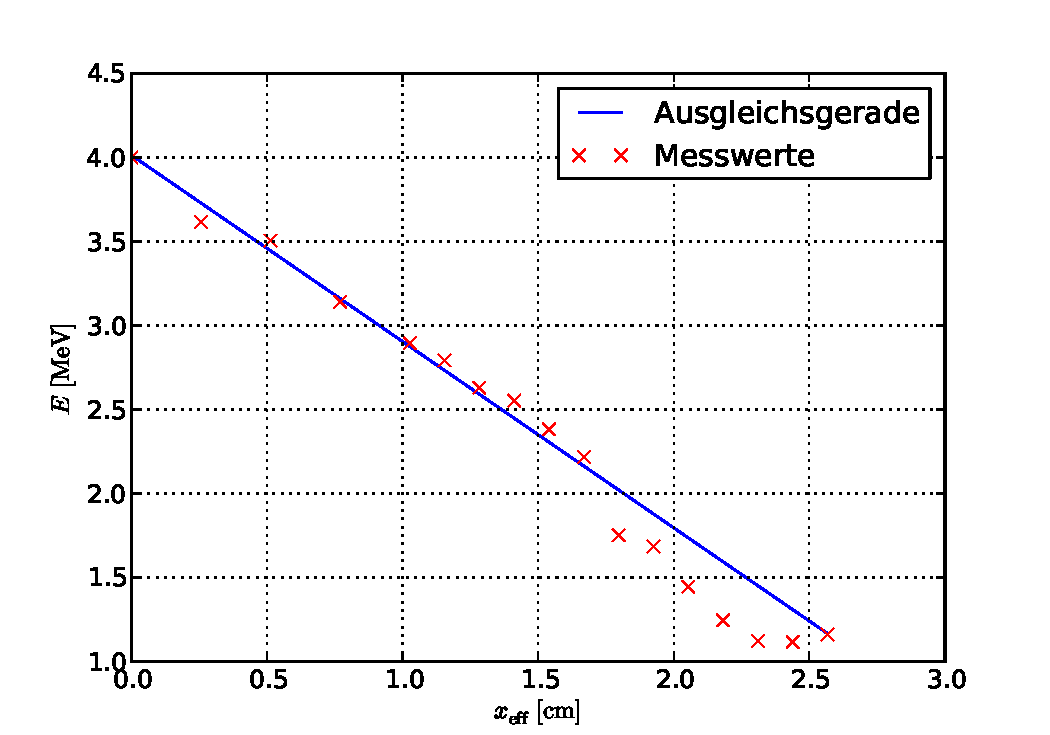
\includegraphics[width = 13cm]{img/energie1.pdf}
			\caption{Lineare Ausgleichsgerade f"ur Energie $E$ und L"ange $x_\mathrm{eff}$ bei einer Basisl"ange von $x_{0,1}$ \label{fig:energie1}}
		\end{figure}

		\begin{figure}[h]
			\centering
			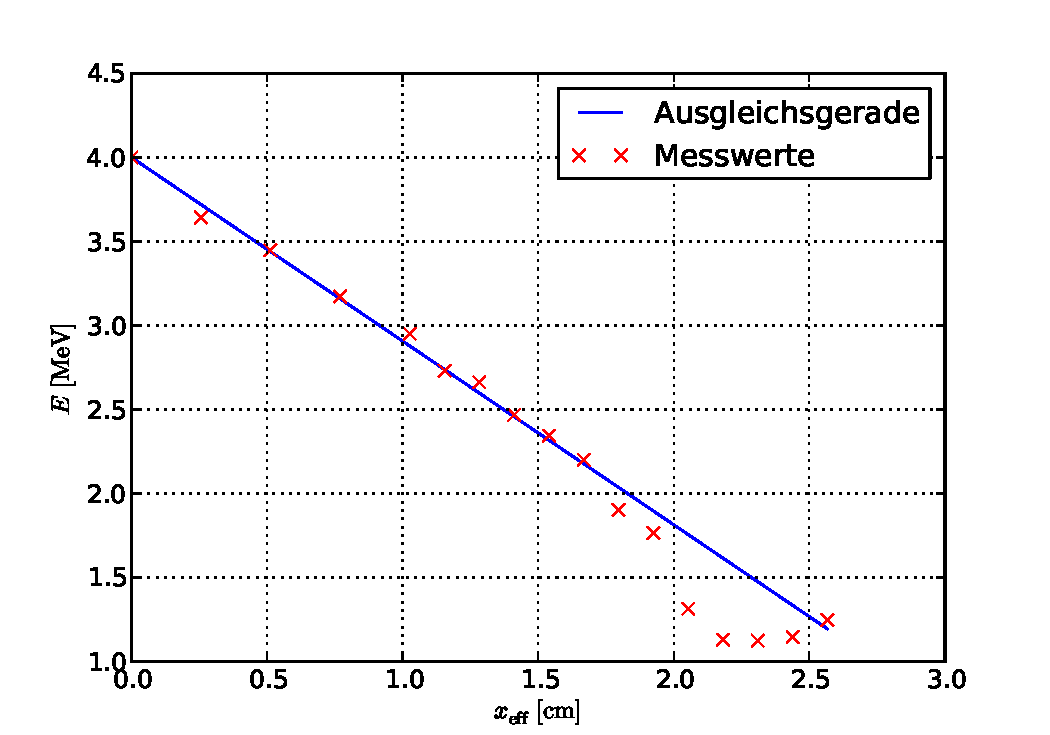
\includegraphics[width = 13cm]{img/energie2.pdf}
			\caption{Lineare Ausgleichsgerade f"ur Energie $E$ und L"ange $x_\mathrm{eff}$ bei einer Basisl"ange von $x_{0,1}$ \label{fig:energie2}}
		\end{figure}

		\clearpage

	\subsection{Statistik des radioaktiven Zerfalls}
	\label{subsec:statistik}
		Tabelle \ref{table:messung2} enth"alt die Z"ahlraten dieser Messung.
		Die Messwerte sind im Anhang aufgef"uhrt.
		Es wurde jeweils "uber $T = \SI{10}{\second}$ gemessen.
		Zur Erstellung eines Histogramms wurde die Gr"o"se $\Delta N$ der H"aufigkeitsbereiche auf

		\begin{equation*}
			\Delta N = \SI{9.75}{}
		\end{equation*}

		festgelegt.
		Hierdurch erh"alt man acht Bereiche, in denen Zerf"alle gemessen werden.
		Der Erwartungswert $\overline{z}$, sowie die Varianz $\sigma_z$ betragen

		\begin{eqnarray*}
			\overline{z} & = & \SI{506.613}{\per \second} \,, \\
			\sigma_z & = & \SI{290.672}{\per \second} \,.
		\end{eqnarray*}

		Die Abbildungen \ref{fig:verteilungGauss} und \ref{fig:verteilungPoisson} beinhalten die Histogramme mitsamt einer Gausskurve, bzw. einer Poissonverteilung.

		\begin{table}[h!]
			\begin{center}
				\caption{Messwerte zur Ermittlung der Statistik des radioaktiven Zerfalls \label{table:messung2}}
				\begin{tabular}{|c|c|c|c|c|c|c|c|c|c|}
					\hline
						\multicolumn{10}{|c|}{$z \left[\SI{}{\per \second}\right]$} \\
					\hline 
					\hline
						\SI{522.1}{} & \SI{507.0}{} & \SI{494.0}{} & \SI{513.6}{} & \SI{512.2}{} & \SI{475.3}{} & \SI{480.3}{} & \SI{527.8}{} & \SI{504.5}{} & \SI{523.9}{} \\
\SI{494.0}{} & \SI{508.0}{} & \SI{493.3}{} & \SI{473.1}{} & \SI{490.5}{} & \SI{476.2}{} & \SI{513.8}{} & \SI{507.5}{} & \SI{510.4}{} & \SI{518.9}{} \\
\SI{508.4}{} & \SI{500.4}{} & \SI{522.1}{} & \SI{522.2}{} & \SI{505.2}{} & \SI{498.5}{} & \SI{488.8}{} & \SI{491.9}{} & \SI{535.1}{} & \SI{500.7}{} \\
\SI{503.4}{} & \SI{501.2}{} & \SI{540.2}{} & \SI{529.4}{} & \SI{527.1}{} & \SI{546.4}{} & \SI{530.9}{} & \SI{495.3}{} & \SI{485.1}{} & \SI{499.5}{} \\
\SI{538.1}{} & \SI{512.0}{} & \SI{517.3}{} & \SI{506.3}{} & \SI{510.9}{} & \SI{487.5}{} & \SI{536.0}{} & \SI{513.7}{} & \SI{517.6}{} & \SI{507.8}{} \\
\SI{523.1}{} & \SI{491.8}{} & \SI{517.6}{} & \SI{520.1}{} & \SI{520.2}{} & \SI{517.8}{} & \SI{477.0}{} & \SI{491.1}{} & \SI{497.7}{} & \SI{524.8}{} \\
\SI{523.3}{} & \SI{525.1}{} & \SI{488.3}{} & \SI{491.9}{} & \SI{521.1}{} & \SI{524.1}{} & \SI{516.7}{} & \SI{480.3}{} & \SI{481.2}{} & \SI{520.7}{} \\
\SI{529.8}{} & \SI{479.6}{} & \SI{541.0}{} & \SI{489.8}{} & \SI{493.1}{} & \SI{523.9}{} & \SI{490.1}{} & \SI{505.1}{} & \SI{507.1}{} & \SI{538.1}{} \\
\SI{517.4}{} & \SI{483.0}{} & \SI{517.0}{} & \SI{472.6}{} & \SI{534.2}{} & \SI{540.2}{} & \SI{535.0}{} & \SI{527.0}{} & \SI{498.0}{} & \SI{485.0}{} \\
\SI{494.0}{} & \SI{503.7}{} & \SI{509.1}{} & \SI{518.3}{} & \SI{488.5}{} & \SI{486.0}{} & \SI{518.9}{} & \SI{522.2}{} & \SI{499.9}{} & \SI{494.0}{} \\
\SI{492.2}{} & \SI{502.8}{} & \SI{503.2}{} & \SI{526.4}{} & \SI{525.5}{} & \SI{495.7}{} & \SI{528.6}{} & \SI{485.2}{} & \SI{513.7}{} & \SI{504.2}{} \\
\SI{520.9}{} & \SI{487.5}{} & \SI{494.6}{} & \SI{485.2}{} & \SI{483.7}{} & \SI{493.1}{} & \SI{501.8}{} & \SI{481.2}{} & \SI{499.4}{} & \SI{517.5}{} \\
\SI{505.3}{} & \SI{534.8}{} & \SI{500.6}{} & \SI{504.8}{} & \SI{522.8}{} & \SI{527.5}{} & \SI{505.7}{} & \SI{485.9}{} & \SI{490.5}{} & \SI{498.8}{} \\
\SI{518.5}{} & \SI{508.0}{} & \SI{496.4}{} & \SI{488.3}{} & \SI{494.2}{} & \SI{512.9}{} & \SI{514.8}{} & \SI{498.2}{} & \SI{508.6}{} & \SI{510.4}{} \\
\SI{488.4}{} & \SI{526.5}{} & \SI{507.7}{} & \SI{498.7}{} & \SI{506.1}{} & \SI{481.5}{} & \SI{489.2}{} & \SI{485.3}{} & \SI{518.5}{} & \SI{499.7}{} \\










					\hline 
				\end{tabular}
			\end{center}
		\end{table}

		\clearpage

		\begin{figure}[h!]
			\centering
			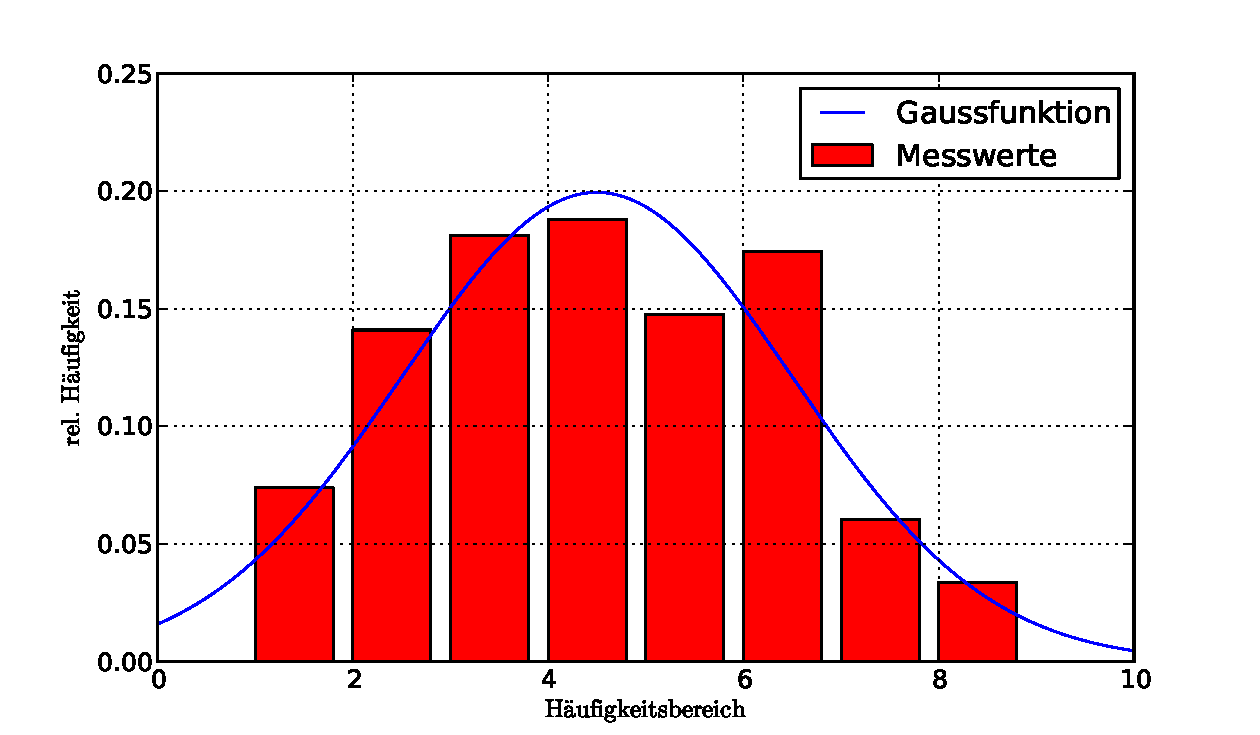
\includegraphics[width = 14cm]{img/verteilungGauss.pdf}
			\caption{Statistik des radioaktiven Zerfalls in Gegen"uberstellung zur Gausskurve \label{fig:verteilungGauss}}
		\end{figure}

		\begin{figure}[h!]
			\centering
			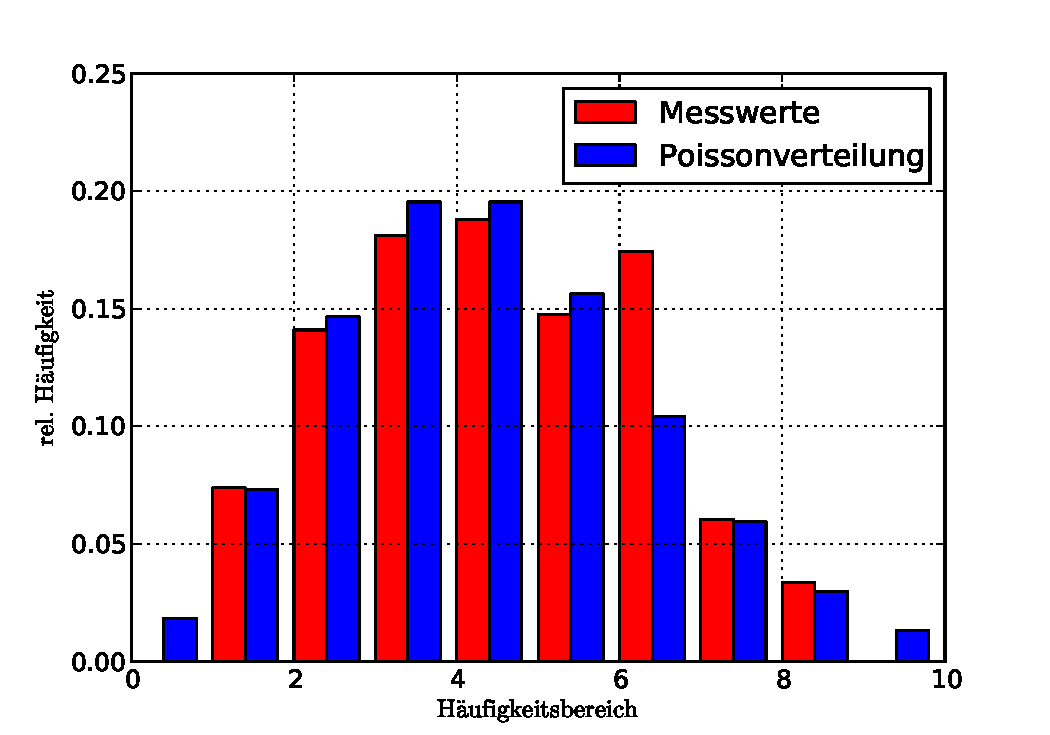
\includegraphics[width = 14cm]{img/verteilungPoisson.pdf}
			\caption{Statistik des radioaktiven Zerfalls in Gegen"uberstellung zur Poissonverteilung \label{fig:verteilungPoisson}}
		\end{figure}

	\clearpage